\begin{minipage}[t]{0.5\linewidth}
	\subsection*{Partie A}
\begin{enumerate}
	\item On lit sur le graphique que l'image de 3,6 cm par cette fonction est environ 200 cm$^3$.
	\item On lit sur le graphique que l'antécédent de \np[cm^3]{660} par cette fonction est environ 5,4 cm.
\end{enumerate}
\end{minipage}
\hfill~
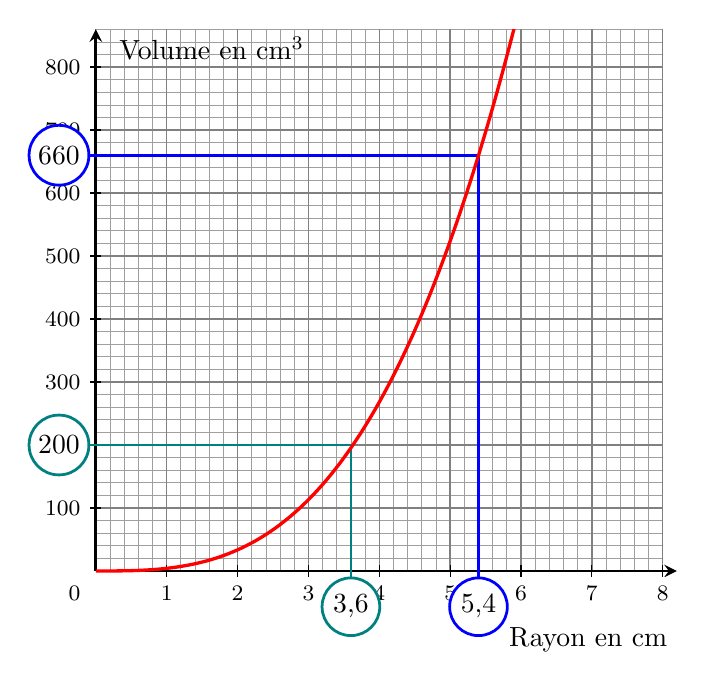
\begin{tikzpicture}[x=9mm,y=0.08mm,baseline={(vol.base)},> =stealth]
	\draw [color = gray!75, line width = 0.25pt, xstep=0.2, ystep = 20] (0,0) grid (8,860);
	\draw [color = gray, line width = 0.5pt, xstep=1, ystep = 100] (0,0) grid (8,860);
	\draw[->,line width=1pt] (0,0) -- (8.2,0);
	\node[left] at (8.2,-25pt) {Rayon en cm};
	\foreach \x in {1,...,8}
	\draw[shift={(\x,0)},color=black] (0pt,2pt) -- (0pt,-2pt) node[below, fill = white] {\footnotesize $\np{\x}$};
	\draw[->,line width=1pt] (0,0) -- (0,860);
	\node[right] (vol) at (5pt,830) {Volume en $\mathrm{cm}^3$};
	\foreach \y in {100,200,...,800}
	\draw[shift={(0,\y)},color=black] (2pt,0pt) -- (-2pt,0pt) node[left, fill = white] {\footnotesize $\np{\y}$};
	\draw[color=black] (-2pt,-2pt) node[below left] {{\footnotesize 0}};
	\draw[teal,line width=1pt] (3.6,-2pt) node[below,circle,fill=white, draw,text=black,inner sep=2pt]{3,6} -- (3.6,200) -- (-2pt,200) node[left,circle,fill=white, draw,text=black,inner sep=2pt]{200};
	\draw[blue,line width=1pt] (5.4,-2pt) node[below,circle,fill=white, draw,text=black,inner sep=2pt]{5,4} -- (5.4,660) -- (-2pt,660) node[left,circle,fill=white, draw,text=black,inner sep=2pt]{660};
	\clip (0,-2pt) rectangle (8,860);
	\draw[line width=1.2pt,color=red,smooth,samples=100,domain= 0:6] plot(\x,{4.18879*\x*\x*\x});
\end{tikzpicture}

\needspace{10\baselineskip}
% saut de page si moins de 10 lignes disponibles
\subsection*{Partie B}
\begin{enumerate}
	\item $\mathcal{V}=\dfrac{4}{3}\times \pi\times 2,5^3\approx \np[]{65.45}$: le volume d'une boule, arrondi à l'unité, est d'environ \np[~cm^3]{65}.
	\item $\dfrac{\np{1000}}{65}\approx 15,4$

	Donc on peut fabriquer au maximum 15 boules avec \np[~cm^3]{1000} de plastique.
	\item On construit un tableau de proportionnalité :
	\quad
	\begin{tabular}{c|c|c}
	masse en g& \np{0.9} &$x$ \\\hline
	volume en cm\up{3}& 1 &65  \\
\end{tabular}

	$0,9\times 65= 58,5$ g.

	Donc la masse d'une boule est d'environ \np[~g]{59}. %arrondir à l'entier car 65 est déjà arrondi à l'entier
\end{enumerate}

\needspace{10\baselineskip}
% saut de page si moins de 10 lignes disponibles
